% ============================================================================
%  6. ỨNG DỤNG, KẾT LUẬN VÀ HƯỚNG PHÁT TRIỂN
% ============================================================================
\section{Ứng dụng, kết luận và hướng phát triển}
\label{sec:ket-luan}

\subsection{Ứng dụng đã triển khai}

Cơ sở tri thức và động cơ suy diễn được đóng gói thành một ứng dụng web (FastAPI) dùng chung
một lõi với bộ đánh giá, nên số liệu in ra luôn đến từ đúng mã nguồn đang phục vụ giao diện.

\begin{table}[H]
\centering
\caption{Các mặt tiếp cận của hệ thống}
\label{tab:mat-tiep-can}
\small
\renewcommand{\arraystretch}{1.22}
\begin{tabularx}{\textwidth}{@{}>{\raggedright\arraybackslash}p{3.4cm} >{\raggedright\arraybackslash}p{5.2cm} L@{}}
\toprule
\textbf{Mặt tiếp cận} & \textbf{Đường dẫn / lệnh} & \textbf{Dùng cho} \\
\midrule
Giao diện tra cứu      & \code{/tra-cuu?q=} · \code{/dieu-khoan/\{id\}} & Người dùng cuối --- tra cứu kèm nguyên văn điều khoản và căn cứ \\
Xem theo mốc thời gian & \code{/hieu-luc?dk=} · bộ lọc \code{ngay=YYYY-MM-DD} & So câu chữ trước và sau sửa đổi --- ``tại thời điểm $t$ thì sao'' \\
Duyệt theo chủ đề      & \code{/chu-de?}\allowbreak\code{linh\_vuc=\&nhom=} & Người học luật --- đọc có hệ thống theo 6 lĩnh vực \\
Bảng chỉ số            & \code{/chi-so} & Người chấm --- xem chỉ số đo trực tiếp trên hệ \\
API JSON               & \code{/api/ask} · \code{/api/docs} (OpenAPI) & Tích hợp vào ứng dụng khác \\
Đóng gói Docker        & \code{docker compose up giao-dien} & Chạy lại toàn bộ mà không cần cài Python \\
\bottomrule
\end{tabularx}
\end{table}

Giao diện đáp ứng được cả màn hình nhỏ: dưới 720~px thanh bên chuyển thành thanh tab đáy, dùng
chung đường dẫn chứ không có bản mobile riêng. Hai bộ lọc \code{ngay} (mốc thời gian) và
\code{pt} (phương tiện) dùng chung trên mọi màn hình. Các hình dưới đây chụp trực tiếp từ ứng
dụng đang chạy trên máy cá nhân.

\begin{figure}[H]
\centering
\fbox{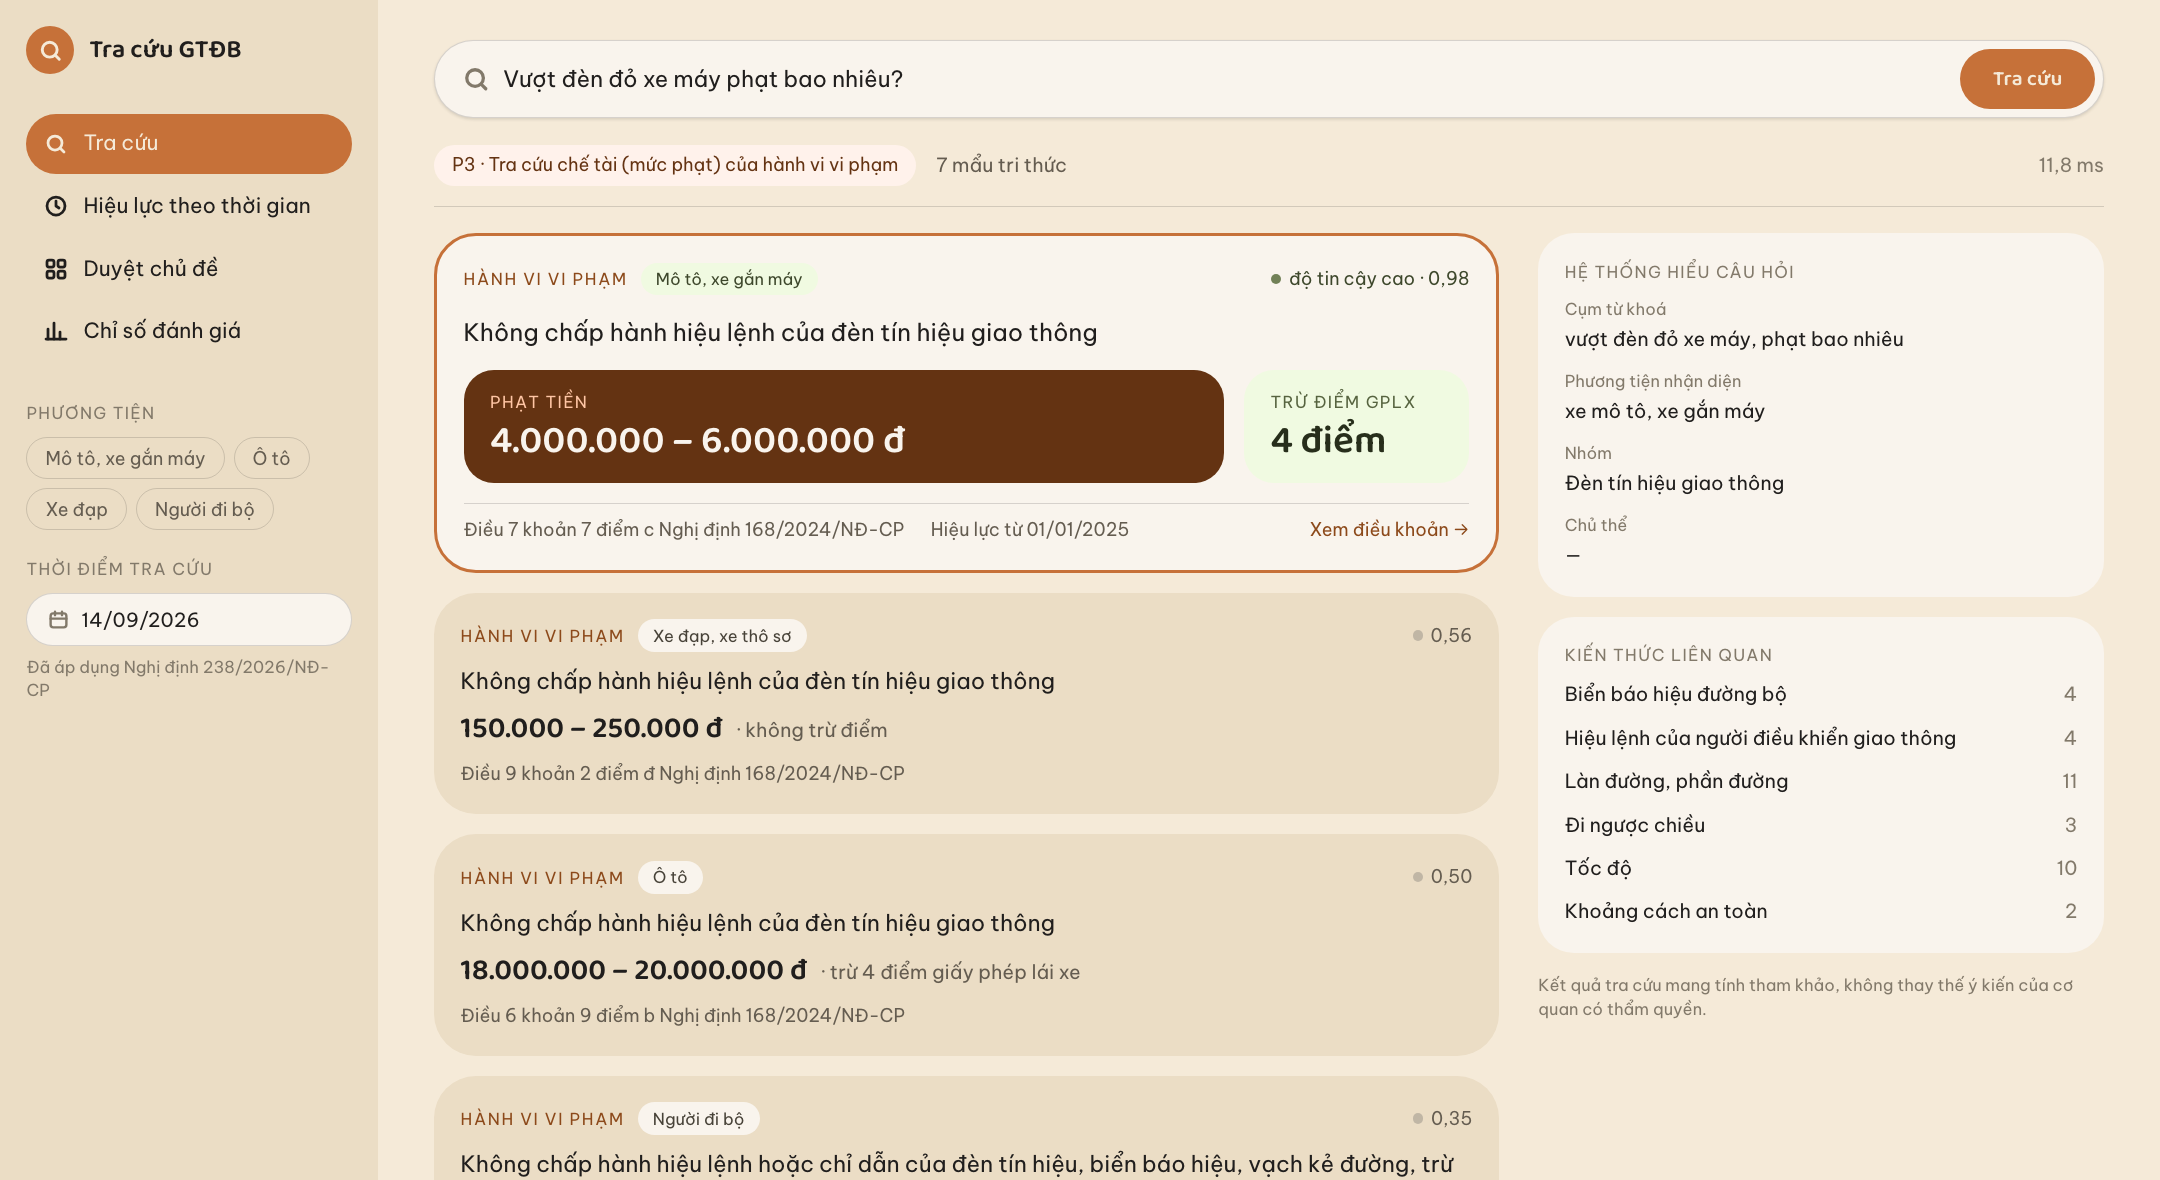
\includegraphics[width=0.97\textwidth]{figures/ui_tra_cuu.png}}
\caption{Màn hình tra cứu với câu hỏi ``Vượt đèn đỏ xe máy phạt bao nhiêu?'': kết quả hạng 1
đúng khung Điều 7 khoản 7 điểm c NĐ 168/2024, kèm mức phạt, điểm trừ GPLX, căn cứ và phần
``hệ thống hiểu câu hỏi'' (cụm từ khoá, phương tiện, nhóm)}
\label{fig:ui-tra-cuu}
\end{figure}

\begin{figure}[H]
\centering
\fbox{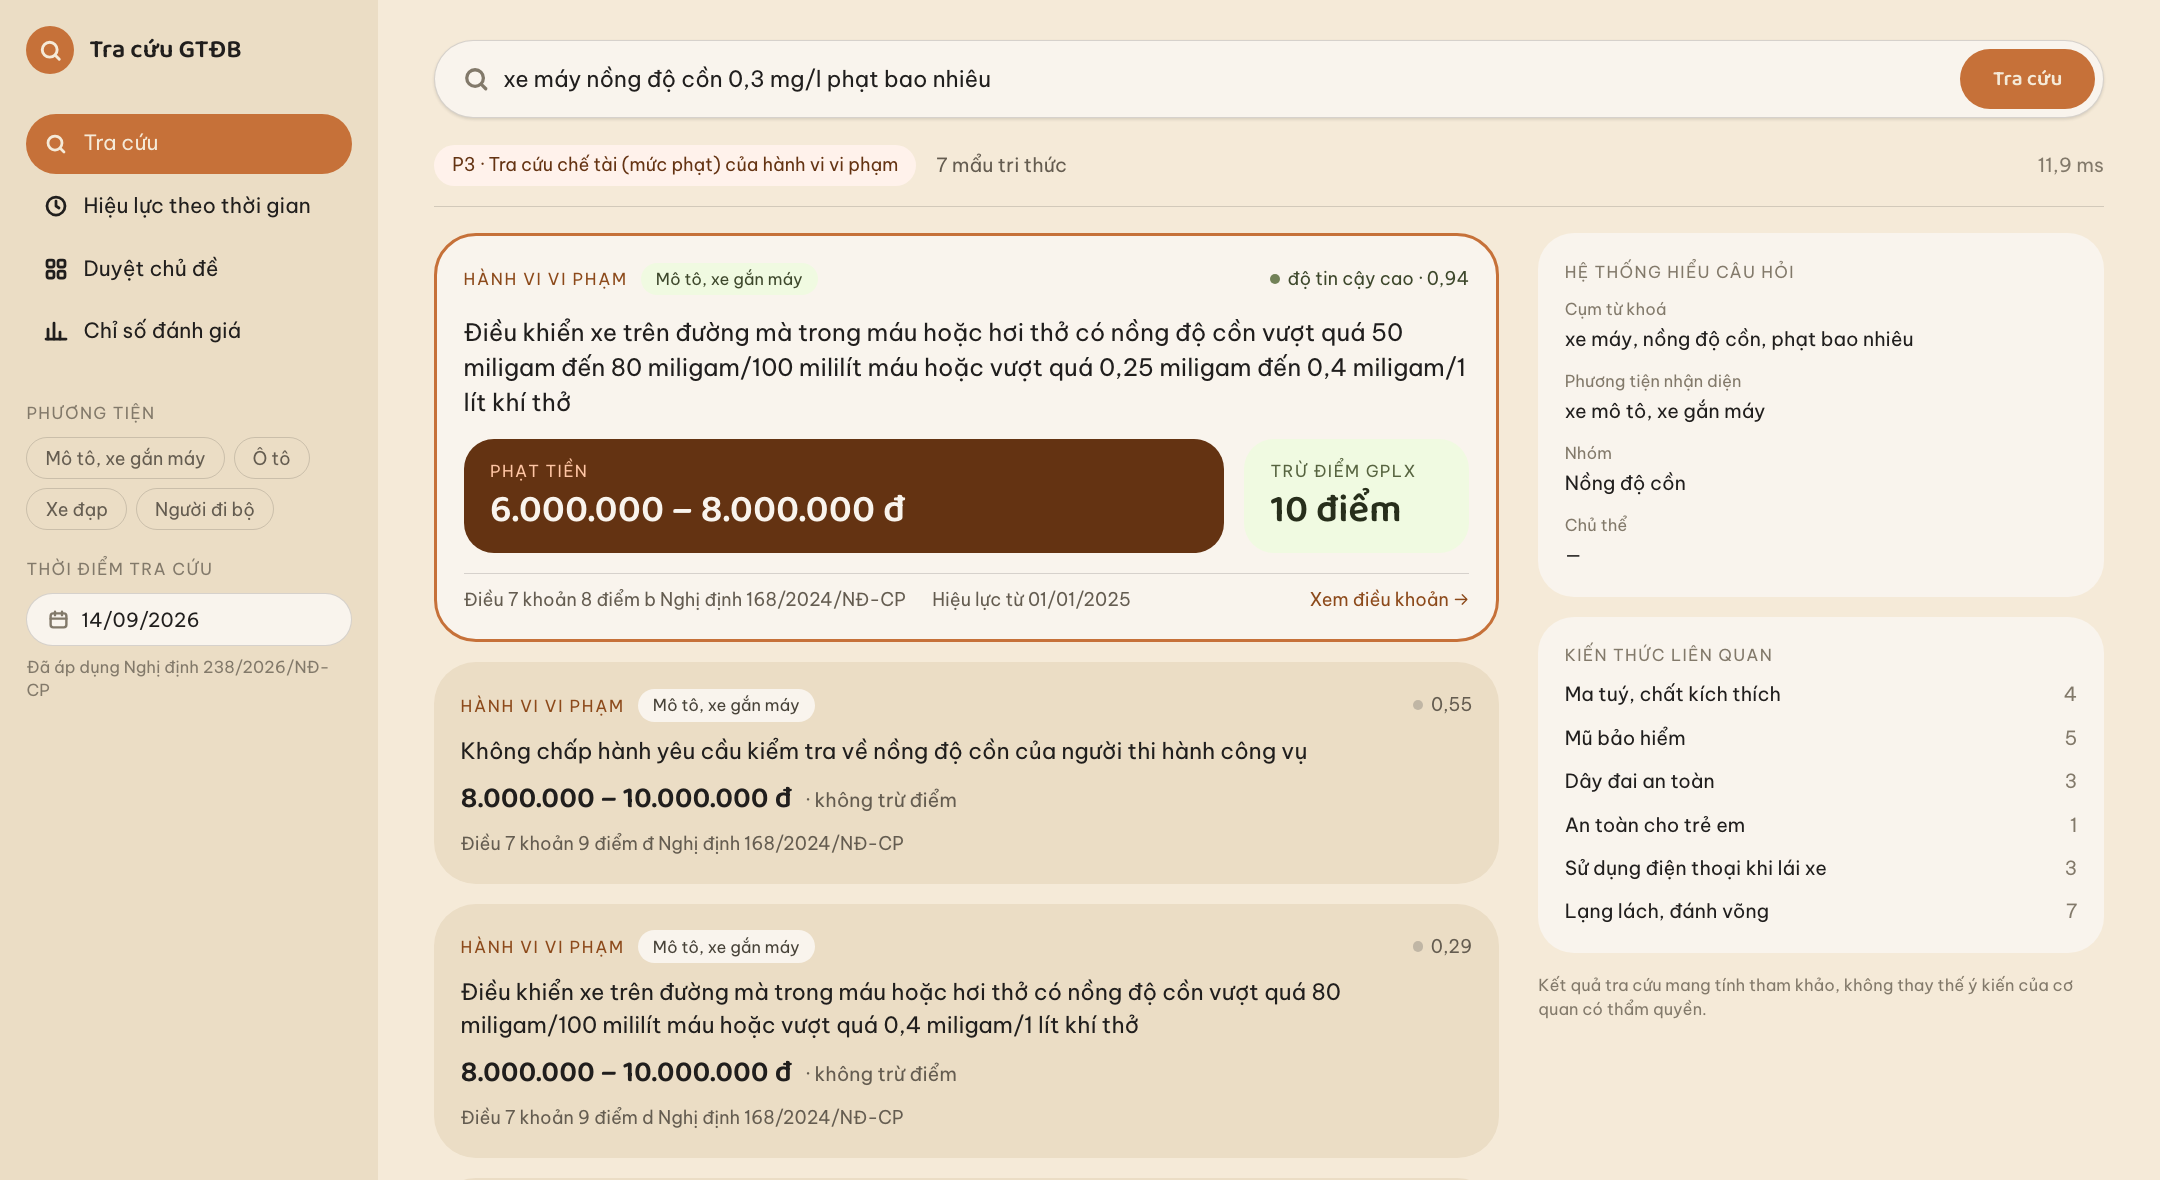
\includegraphics[width=0.97\textwidth]{figures/ui_so_hoc.png}}
\caption{Suy diễn số học: với ``xe máy nồng độ cồn 0,3 mg/l'', khung ``vượt quá 0,25 đến 0,4
miligam/1 lít khí thở'' (6--8 triệu đồng, trừ 10 điểm) được đẩy lên đầu}
\label{fig:ui-so-hoc}
\end{figure}

\begin{figure}[H]
\centering
\fbox{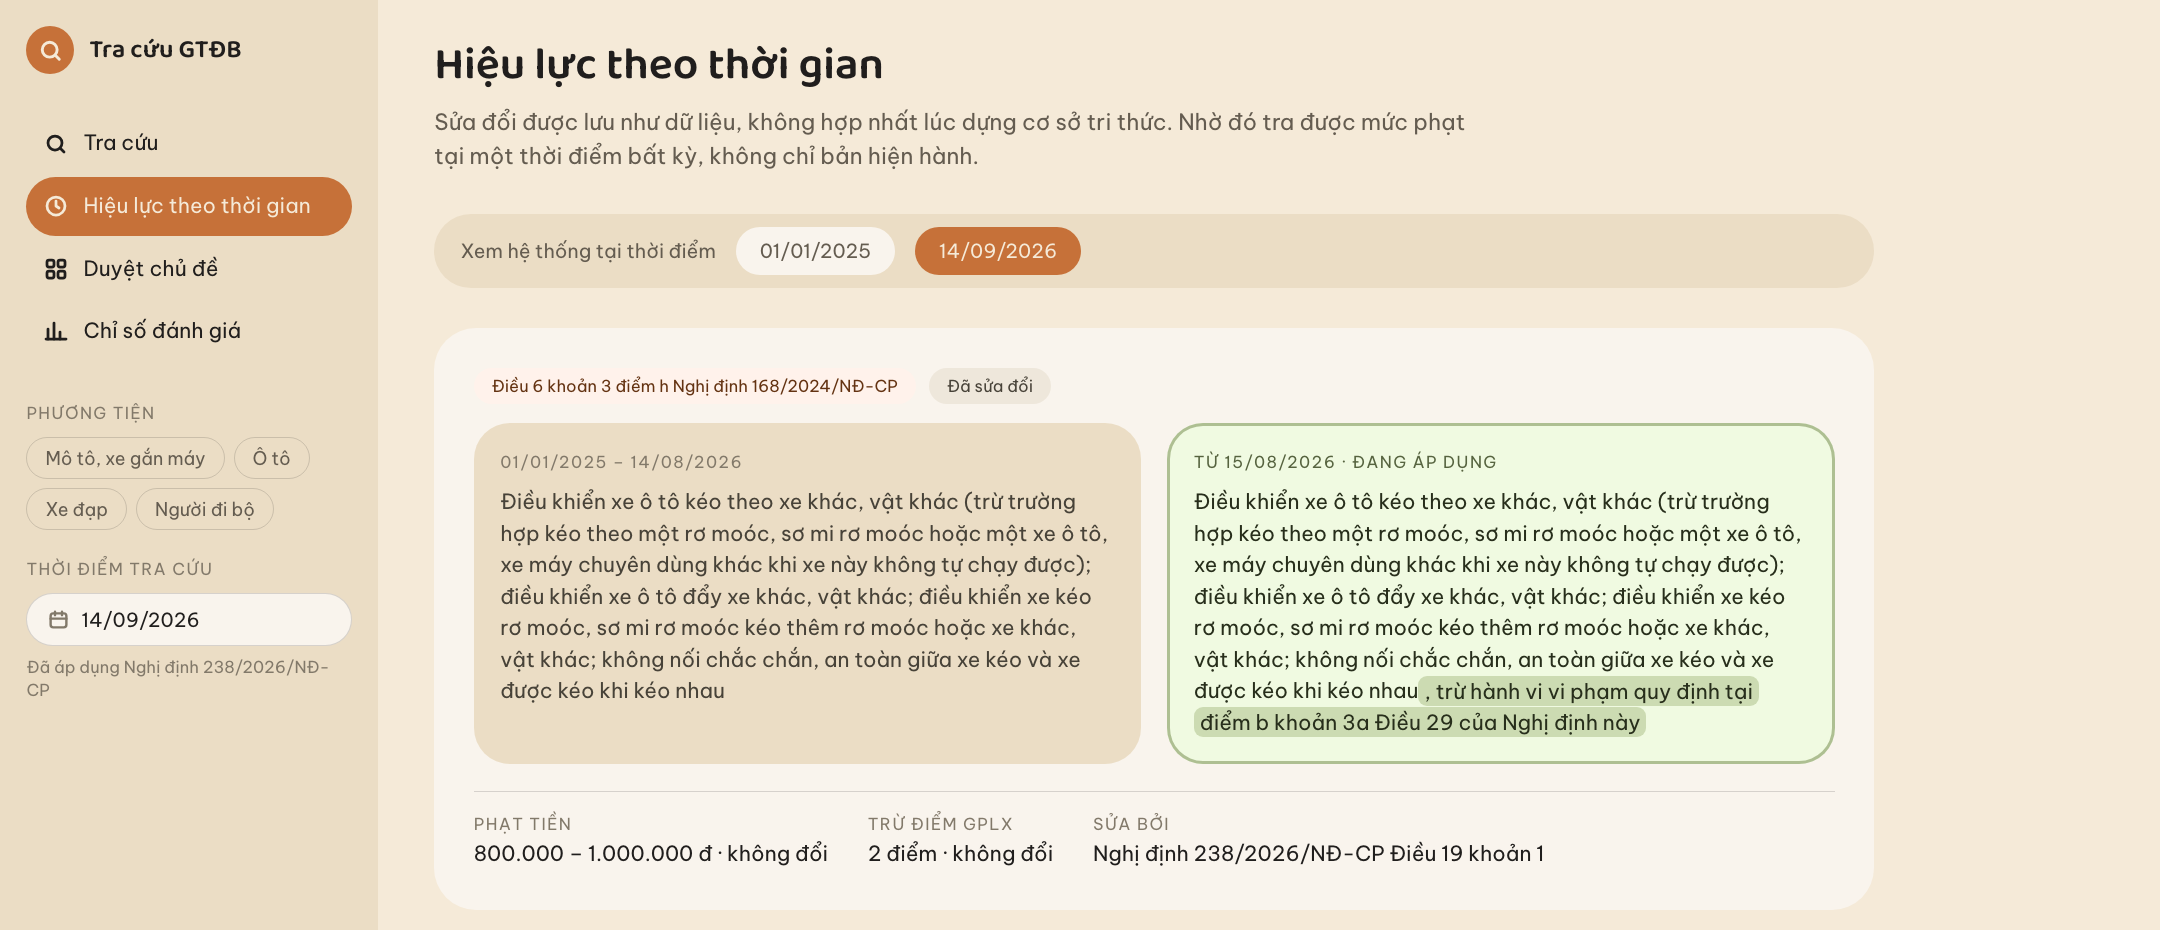
\includegraphics[width=0.97\textwidth]{figures/ui_hieu_luc.png}}
\caption{Màn hình hiệu lực theo thời gian: đối chiếu nguyên văn một điều khoản trước và sau
khi Nghị định 238/2026/NĐ-CP có hiệu lực (15/8/2026)}
\label{fig:ui-hieu-luc}
\end{figure}

Giá trị sử dụng thực tế nằm ở ba chỗ: câu trả lời luôn kèm căn cứ tới mức điều -- khoản -- điểm
nên kiểm chứng được; tra cứu được theo mốc thời gian nên không đưa nhầm quy định đã hết hiệu
lực; và toàn bộ chạy cục bộ trong khoảng 6~ms mỗi truy vấn, không gửi câu hỏi của người dân ra
dịch vụ ngoài.

\subsection{Hạn chế}
\label{sec:han-che}

Mọi hạn chế dưới đây đều đã \textbf{đo được} và phần lớn được khoá lại bằng test \code{xfail}
trong kho mã, không phải phỏng đoán. Nhóm trình bày cả những hướng đã thử và đã bác bỏ, vì một
kết quả âm có số đo cũng là kết quả.

\subsubsection{Chưa từ chối được truy vấn ngoài lĩnh vực}

Ở cấu hình mặc định, hỏi ``cách nấu phở bò'' thì hệ thống vẫn trả về tri thức giao thông: cả
\textbf{40/40} truy vấn ngoài miền đều được trả lời thay vì bị từ chối. Nguyên nhân đã khoanh
vùng: đặc trưng TF-IDF quá yếu để tách miền --- 56/120 câu hợp lệ chấm điểm thấp hơn hoặc bằng
truy vấn rác, nên không tồn tại ngưỡng nào tách được hai phân bố.

\begin{table}[H]
\centering
\caption{Khả năng tách miền của bốn tín hiệu (120 câu trong miền · 40 truy vấn ngoài miền)}
\label{tab:tach-mien}
\renewcommand{\arraystretch}{1.2}
\begin{tabularx}{\textwidth}{@{}L r r r@{}}
\toprule
\textbf{Tín hiệu} & \textbf{AUC} & \textbf{Loại rác khi 0 câu oan} & \textbf{Oan khi loại hết rác} \\
\midrule
TF-IDF thô       & 0,8746 & 7,5\%  & 66,7\% \\
Số keyphrase     & 0,9500 & 0,0\%  & 10,0\% \\
Phủ từ vựng KB   & 0,7243 & 47,5\% & 100,0\% \\
\textbf{Dense embedding} & \textbf{0,9958} & \textbf{77,5\%} & \textbf{5,8\%} \\
\bottomrule
\end{tabularx}
\end{table}

Nhóm đã kiểm chứng đề xuất thay đặc trưng: dense embedding nâng AUC từ 0,8746 lên 0,9958 và
riêng điểm dense loại được 77,5\% truy vấn rác mà không từ chối oan câu hợp lệ nào; bộ lọc kết
hợp keyphrase + dense (ngưỡng 0,45) loại được 92,5\%. Nhưng hai phân bố \emph{vẫn} chồng lấn:
trần điểm dense của truy vấn rác (0,5158) cao hơn sàn điểm của câu hợp lệ (0,3919). Muốn loại
100\% truy vấn rác thì phải chấp nhận từ chối oan 5,8\% câu hợp lệ. Nhóm từ chối đánh đổi đó và
giữ tầng dense ở dạng tuỳ chọn --- mô hình nặng khoảng 470~MB cũng là một lý do. Bản demo mặc
định vì vậy chưa có bộ lọc miền.

\emph{Kết quả âm đáng ghi nhận:} phủ từ vựng cơ sở tri thức là tín hiệu vô dụng cho việc tách
miền (AUC 0,7243, thấp hơn cả TF-IDF thô). Hướng này đã thử và đã bác bỏ.

\subsubsection{Các hạn chế còn lại}

\begin{itemize}
  \item \textbf{Khoảng trống từ vựng là nguồn lỗi lớn nhất:} 15 ca được quy trực tiếp về nguyên
        nhân này, và tính rộng ra thì 27/31 ca chưa tối ưu đều có đặc điểm chung là không cụm từ
        khoá nào của đáp án xuất hiện trong câu hỏi. Đây là hạn chế của dữ liệu chứ không của
        thuật giải.
  \item \textbf{Chưa có tập đánh giá giữ lại:} trọng số hàm điểm được chọn bằng ablation trên
        chính 120 câu hỏi đánh giá, và cổng CI cũng đo trên bộ này. Con số 76,67\% vì vậy là kết
        quả trên bộ câu hỏi dùng trong quá trình phát triển; khả năng khái quát sang câu hỏi mới
        chưa được đo.
  \item \textbf{Bộ câu hỏi chưa phủ đều cơ sở tri thức:} 120 câu chạm tới 115/527 mục tri thức
        truy hồi được (21,8\%); lĩnh vực ``Điều kiện của phương tiện'' bị đánh giá nhẹ hơn tỉ
        trọng của nó.
  \item \textbf{Câu tình huống nhiều vi phạm:} hệ tìm đủ mọi vi phạm ở 9/15 câu P5, nên tổng mức
        phạt có thể thiếu một hành vi.
  \item 12/120 câu hợp lệ không rút được keyphrase nào, nên không thể dùng riêng tín hiệu
        keyphrase làm bộ lọc truy vấn ngoài lĩnh vực.
  \item Chưa mô hình hoá 46 chú thích sửa đổi của Luật 118/2025/QH15 ở mức từng khoản: đã trích
        ra \code{data/raw/luat118\_dieu7\_chu\_thich.json}, nhưng mô hình \code{SuaDoi} hiện chỉ có
        trường theo Nghị định 168 nên chưa biểu diễn được sửa đổi ở tầng luật.
  \item \textbf{Hệ thống không sinh ngôn ngữ tự nhiên:} câu trả lời được ghép từ nguyên văn điều
        khoản. Đây là lựa chọn có chủ đích --- như các số đo ảo giác ở mục~\ref{sec:lien-quan}
        cho thấy, diễn giải lại lời của luật là rủi ro lớn hơn lợi ích về trải nghiệm.
  \item Hỏi nồng độ cồn mà không nêu phương tiện thì hệ trả về khung xe đạp. Về mặt tri thức là
        đúng --- hệ không bịa phương tiện người dùng chưa nói --- nhưng là vấn đề trải nghiệm cần
        giải quyết bằng câu hỏi làm rõ.
  \item Cỡ mẫu 120 câu khiến khoảng tin cậy của các lớp nhỏ rất rộng (P7 với $n = 5$ có KTC
        Top-1 [12\% -- 77\%]), nên không kết luận mạnh được ở mức từng lớp.
\end{itemize}

\subsection{Hướng phát triển}
\label{sec:huong-phat-trien}

\begin{enumerate}
  \item Mở rộng từ điển cụm từ khoá bằng khẩu ngữ thu từ truy vấn thật --- nhắm thẳng vào nhóm lỗi
        L5, nhóm chiếm 15/31 ca chưa tối ưu và là hướng cải thiện rẻ nhất.
  \item Xây một tập câu hỏi giữ lại do người ngoài nhóm soạn, không dùng để chỉnh trọng số, và
        công bố Top-1 trên tập này cạnh con số hiện tại.
  \item Bổ sung tầng hỏi lại khi truy vấn thiếu thông tin bắt buộc (phương tiện, chủ thể) thay vì
        mặc định chọn khung rộng nhất; tách câu tình huống thành từng hành vi trước khi tra.
  \item Thêm tín hiệu phân biệt cho lớp P2: các quy tắc gần nghĩa cần được tách bằng quan hệ trong
        đồ thị $R$, không chỉ bằng điểm tương đồng văn bản.
  \item Tổng quát hoá mô hình \code{SuaDoi} để biểu diễn được sửa đổi ở cả tầng luật và tầng nghị
        định, khép nốt 46 chú thích còn lại --- bước tiến gần hơn tới mô hình sửa đổi hình thức
        của Governatori và cộng sự~\cite{governatori}.
  \item Đưa tầng dense embedding vào bản triển khai có tài nguyên, kèm ngưỡng hai mức: từ chối
        khi chắc chắn, cảnh báo thay vì chặn khi nghi ngờ.
  \item Về dài hạn, công bố cơ sở tri thức và bộ câu hỏi như một tài nguyên mở cho lĩnh vực giao
        thông đường bộ Việt Nam.
\end{enumerate}

\subsection{Kết luận}

Nhóm đã xây dựng hoàn chỉnh một hệ tra cứu kiến thức pháp luật giao thông đường bộ theo đúng
yêu cầu Đề tài 4: cơ sở tri thức có cấu trúc gồm 73 khái niệm, 482 quan hệ, 109 quy tắc, 345
hành vi vi phạm và 1.674 cụm từ khoá; bộ dữ liệu 120 câu hỏi có đáp án chuẩn; thuật giải xử lý
truy vấn sáu bước; và một giao diện tra cứu chạy được.

Về số đo, hệ thống đạt độ chính xác phân lớp 95,83\%, Top-1 76,67\% (KTC 95\% [68,3\% --
83,3\%]), Top-5 95,00\% và MRR 0,8384, thời gian trả lời trung bình 6,2~ms trên máy cá nhân,
hoàn toàn không phụ thuộc dịch vụ ngoài. Thí nghiệm loại bỏ thành phần chứng minh từng phần của
hàm điểm đều đóng góp thực chất, và kiểm định McNemar ($p = 0{,}000488$) khẳng định bước suy
diễn số học tạo khác biệt có ý nghĩa thống kê chứ không phải may rủi.

So với các công trình khảo sát ở mục~\ref{sec:lien-quan}, đóng góp riêng của đồ án nằm ở chỗ
ghép được ba thứ vốn tách rời: mô hình tri thức tường minh theo hướng
Legal-Onto~\cite{legalonto}, suy diễn số học để tính chế tài, và mô hình hoá hiệu lực theo thời
gian ở mức khoản --- trên khung pháp lý giao thông đường bộ 2024--2026.

Điều nhóm thấy đáng giá nhất không phải là con số Top-1 mà là \textbf{kỷ luật đo đạc}: mọi
khẳng định trong báo cáo này đều sinh ra từ một lệnh chạy lại được, mọi hạn chế đều có số đo
kèm theo, mọi tỉ lệ đều kèm khoảng tin cậy, và những hướng đã thử rồi bác bỏ đều được ghi lại
thay vì giấu đi.
